
\section{Related Works}
\label{sec:literature}

\subsection{Systematic Literature Review process}

This SLR aims at tackling RQ1 and RQ2. More precisely, the following research questions will be answered:

\begin{itemize}
    \item [RQ1] What is the current state-of-the-Art for DAG tasks scheduling ?        
    \item [RQ2] What machine learning  techniques are used for DAG task scheduling ?
\end{itemize}
It will also be shown how the literature doesn't provide 
a complete answer to RQ3, hence the contributions of this paper.\\

From these research questions, several concepts have been isolated,
namely, time-triggered tasks, the nature of the system (real-time multicore system),
the scheduling of tasks, DAG tasks, and machine learning.
The recording of the search results were done using the BibTeX LateX plugin
combine with the google scholar "cite" feature.

Searching was conducted using the IEEE and ACM databases.
According to the concepts identified above, 
the keyword chain used for searching was 
"("real-time" OR "real time") AND 
"system" AND ("time-triggered" OR "time triggered" OR "DAG" OR "Directed Acyclic Graph" OR "event chain" OR "event-chain") 
AND "task" 
AND ("scheduling" OR "scheduler" OR "schedule") 
AND ("multi-processors" OR "multi-cores" OR "multi processors" OR 
"multi cores" OR "multi-processor" OR "multi processor" OR 
"multi-core" OR "multi core")".
             EC1    EC2    EC3
1,259 -> 515 -> 403 -> 101 -> 19 --> 17
The search produced 1,259 results on the IEEE database
which was reduced tp 515 papers when considering only 
articles published in the past 5 years.

Then the following exclusion criterias were used to filter out 
the rest of the articles, bringing the number of papers down to 19
(see Figure \ref{fig:slr_process}).

\begin{itemize}{}{}
    \item [EC1] Not focusing on homogeneous multicores and hard RTS
    \begin{list}{}{}
        \item "Heterogeneous" not in the title nor the abstract.
        \item "mixed critical*" not in the title nor the abstract
    \end{list}
    
    \item [EC2] Not focusing on scheduling
    \begin{list}{}{}        
        \item "scheduling" or "scheduler" or "schedule" in the title 
        \item "energy" not in the title
        \item Focus on conference and journal papers
    \end{list}

    \item [EC3] Not focusing on real-time systems, not proposing a scheduling algorithm, not using DAG or event-chain tasks.
\end{itemize}

\begin{figure}[htbp]
    \centering
    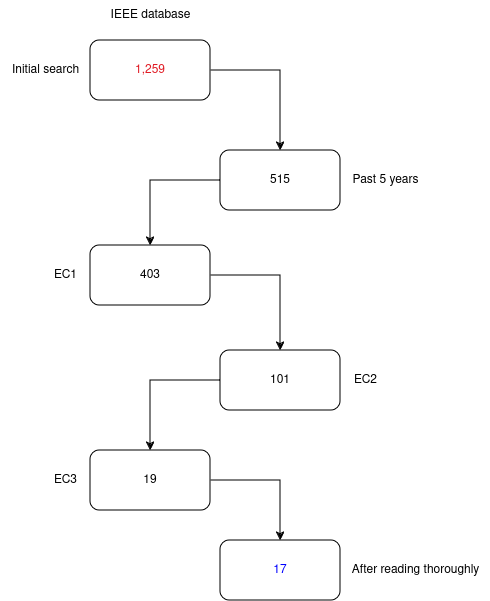
\includegraphics[width=\linewidth]{images/slr_process.png}
    \caption{SLR process diagram. EC stands for Exclusion Criteria,
    which are listed above.}
    \label{fig:slr_process}
\end{figure}


\subsection{Findings of the Literature Review}

\subsubsection{Non-Machine Learning techniques}
~


\citet{guan2021DAGfluid} 
use fluid scheduling to schedule multiple DAG tasks
on a multicore system. 
Fluid scheduling has been used in previous work for independent
time-triggered task scheduling\cite{baruah1993PFair}\cite{cho2006LLREF} 
but very few consider DAG tasks. Fluid-scheduling is known for producing optimal scheduling algorithms.
Their method decomposes a DAG task into several sequential segments
in which the subtasks will execute according to the fluid scheduling 
model. Although their algorithm significantly outperforms
existing algorithms, the main limitation that is common to all fluid-based
scheduling algorithm is the runtime overhead induced by the fluid-scheduling model.
Although authors in \cite{guan2021DAGfluid} briefly explain how 
to transform their scheduling algorithm to a non-fluid one for practical implementation,
they do not evaluate the overhead caused by the frequent task migrations
and preemptions. This overhead can lead to deadline misses
on systems where the migration cost is high which is why it is important,
especially with fluid-based algorithms, to consider this overhead\cite{migrationCostFairSched}.
 Also, their algorithm only considers DAG task with implicit deadlines
(D = T) which makes the response-time analysis simpler but to the cost
of not covering all types of tasks that can execute on real-time systems.

As a follow up, \citet{GuanFluidDag2022} 
extend the fluid scheduling algorithm in \cite{guan2021DAGfluid}
to constrained and arbitrary deadline tasks,
especially focusing on DAG tasks with a deadline greater than their period,
thus generalizing their previous fluid algorithm
to all types of periodic tasks.
Their main contributions are their new scheduling algorithm that 
performs better than existing methods in terms of acceptance ratio,
and producing the first theoretical capacity bound for DAG tasks
with deadlines greater than their periods.
However, the authors still don't provide any evaluation 
on the amount of runtime overhead their scheduling algorithm implementation
produces which generally lowers the actual acceptance ratio
of the algorithm. 

Instead of considering fluid-scheduling,
a popular scheduling method is federated scheduling.
Federated scheduling is based on the idea
of assigning heavy tasks ($U > 1$) to multiple cores
for the whole duration of the tasks' executions,
and assigning light tasks ($U \le 1$) to execute on
cores that have not been assigned a heavy task.
Although it is popular, it suffers from a resource wasting problem,
especially when the difference between the critical path's length 
and the deadline is small,
which many papers aim at solving
\cite{Guan2023FederatedNew}
\cite{jiangUtilTensityBound}
\cite{JiangVirtuallyFederatedSched2021}
\cite{Jiang2023SchedVirtualProcs}
\cite{Kobayashi2023FedBundledDagsched}
\cite{He2023DegreeOfParallelism}.

\citet{jiangUtilTensityBound}, for instance, 
consider federated scheduling and GEDF
and introduces a better metric called the util-tensity bound
that extends the concept of capacity bound
to have a better schedulability test.
Based on this newly derived bound, the authors 
propose an extension to the classic federated algorithm,
with very low tensity tasks being scheduled with GEDF, 
tasks with high-utilization and relatively high tensities are scheduled
using the classic federated scheduling and low utilization
tasks with relatively high tensities are scheduled using partitioned-EDF.
Their algorithm, based on their newly derived bound, effectively improves
the system schedulability of DAG tasks and reduces the resource wasting 
problem of federated scheduling. The main limitation
of this paper is that they only consider GEDF 
for their util-tensity bound and also only consider implicit deadline DAG tasks
which doesn't represent tasks that need to have a deadline 
lower than their period, for example.

This problem of resource wasting in federated scheduling
is also tackled by \citet{Kobayashi2023FedBundledDagsched}
where they propose a federated and bundled-based scheduling
algorithm which enhances the schedulability of DAG tasks
compared to existing federated scheduling algorithms.
Their method consists of using federated scheduling for
tasks with high critical path to deadline ratio and bundled
scheduling for tasks with low critical path to deadline ratio.
Unfortunately, this paper only looks at 3 DAG tasks to evaluate
their algorithm which is a really small amount and is not 
representative of the different DAG tasks that can exist
and leaves space for observational bias.

\citet{JiangVirtuallyFederatedSched2021}
take another approach by proposing a virtually-federated 
scheduling algorithm that leverages the advantages
of federated scheduling while improving the acceptance 
ratio for DAG tasks, outperforming existing algorithms.
Their approach consists of adding a virtual layer
of processors, on top of physical processors,
and apply their federated-based scheduling algorithm on those virtual processors,
thus enabling tasks to share a physical processor
even though they are assigned to different virtual processors.
The main drawback in \cite{JiangVirtuallyFederatedSched2021}
is that the authors only consider the heavy tasks (i.e., $U > 1$)
and do not take the light tasks into account,
meaning it doesn't consider tasks that only need 
one processor to execute.

To fix this limitation, \citet{Jiang2023SchedVirtualProcs}
extend their previous work\cite{JiangVirtuallyFederatedSched2021}
so that it considers both heavy and light tasks.
The resulting virtually federated scheduling algorithm
clearly outperforms any other federated-based scheduling algorithms
in terms of acceptance ratio.
However, they still only consider implicit or constrained deadline tasks
and they don't provide any evaluation of the run time overhead 
their algorithm might induce, to compare with algorithms currently used
in real-time systems, such as GEDF.


\citet{Guan2023FederatedNew} 
consider arbitrary deadline tasks and especially
DAG tasks that have a deadline that is greater than their period.
They introduce a new federated scheduling algorithm 
that takes those type of tasks into account 
and compare it to existing global or federated scheduling approaches
for arbitrary deadline tasks, significantly outperforming
most of them in terms of acceptance ratio.
Their approach consists of using this new proposed aglgorithm 
for heavy tasks that have a deadline bigger than their period,
then using classic federated scheduling for the heavy tasks with a 
constrained deadline, and finally using EDF-First-Fit (EDF-FF) for the light tasks.
Although the fluid-based method in \cite{GuanFluidDag2022}
outperforms this new federated scheduling algorithm,
the impracticality of fluid-based algorithm makes this algorithm
the current best, in terms of acceptance ratio, for dealing with arbitrary
deadlines. The main limitation of this work 
is that it doesn't tackle the resource wasting problem 
that classical federated scheduling, or their new algorithm, has or can potentially have, but only
focuses on providing an algorithm for arbitrary deadline tasks.

For constrained deadline DAG tasks, 
\citet{He2023DegreeOfParallelism} propose a federated-based
scheduling algorithm that outperforms on average by more than 18\%
previous SOTA\cite{Jiang2023SchedVirtualProcs} in terms of acceptance
ratio, making this work the current SOTA for constrained deadline multi-DAG scheduling.
Their approach uses the notion of degree of parallelism, which they 
define rigorously, to improve the classic federated scheduling way of 
choosing the number of cores to assign each heavy tasks.
They also propose a new response-time bound for constrained deadline DAG tasks
based on this defined notion.
Although their method clearly stands out,
they don't consider intra-task scheduling at all 
when their motivation came from the notion 
of degree of parallelism being used
but wrongly defined in previous intra-task scheduling work\cite{Zhao2022DAGsched}\cite{zhao2020DAGsched}.\\

Federated scheduling isn't the only method used,
\citet{JiangDecompoSchedParallelTask},
for instance, propose a decomposition-based 
approach to schedule multi-DAG tasks as well as 
a metric for testing the schedulability of tasks.
Their decomposition strategy proves to be the most efficient 
, according to the defined metric, and the scheduling algorithm
derived from it shows promising results in terms of
acceptance ratio.
Their decomposition strategy basically works by first 
definin execution segments and then then assigning subtasks 
to those segments using the laxity\footnote{Laxity is the gap between the total execution time of a task (potentially comprising the I/O delays) and its deadline.} of those subtasks so that 
no segments are overloaded with workload.
The main limitation of this work is that 
they only look at GEDF variants for priority assignment 
and do not evaluate their decomposition method
using other scheduling heuristics for multi-DAGs.
Most of the articles presented up to now 
tackle inter-task scheduling, not considering
the intra-task execution schedule.

Indeed, intra-task scheduling\cite{He2019DagIntra}\cite{Xiao2019}
\cite{Shi2024DagExecGroups}\cite{Zhao2024GATDRLmodel}\cite{Lee2021GlobalDagSchedDRL}
\cite{GuanFRTDS2020RL} is often tackled as a separate
problem due to the dependency constraints.

\citet{Xiao2019}, for instance, introduce a scheduling algorithm 
, 'MAS', that shortens the makespan of periodic DAG tasks
compared to the classic EDF dynamic priorty scheduling technique.
Their algorithm is based on a clustering approach, combined with
a technique called task duplication, and evaluate their results
on an actual simulation object for real-time scheduling.
Unfortunately, their evaluation is only based on a single DAG task
and they only compare their algorithm with EDF.
Their algorithm also shows a scalability problem compared to 
other existing algorithm with comparable results.

A scalable way of scheduling sub-tasks of a DAG 
is looking at priority-list scheduling
which \citet{He2019DagIntra} use to propose 
an algorithm that effectively outperforms
other intra-task DAG scheduling algorithms
in terms of makespan.
Their priority assignment algorithm
is based on the length of the paths passing through each vertex.
The longer the maximum length, the higher the priority.
This effectively takes advantage of the inner graph structure
to optimize the intra-task execution order,
which is something that hasn't been done before this work.
Although the authors compare their results with existing
scheduling heuristics, they do not consider 
the, mathematically optimal, ILP method to compare
their makespan results with the mathematically minimum makespan.

This priority-list scheduling approach is also 
used by \cite{Zhao2022DAGsched}, extending their previous work\cite{zhao2020DAGsched}
which develop a priority assignment based on 
the critical-path execution first (CPEF) concept,
effectively outperforming \citet{He2019DagIntra}
in terms of makespan and providing 
a federated-based multi-DAG scheduling algorithm,
compatible with this new priority-list scheduling algorithm.
Their multi-DAG scheduling algorithms also outpeforms 
the multi-DAG algorithm used in \cite{He2019DagIntra}.
Their method uses the vertices in the critical path 
as producers of workload for the parallelizable vertices
to consume.
For multi-DAG they look at assigning processors
to DAG tasks, like in federated scheduling, using 
a parallelism-aware workload distribution model
that uses their Concurrent Producer Consumer (CPC) model
to assign cores while minimizing the inter-task workload interference.
One limitation of their work is that,
although they consider constrained deadlines for the response-time
analysis, they only use implicit deadline DAG tasks 
for evaluating the system schedulability of their multi-DAG 
scheduling algorithm.\\


Those intra-task scheduling papers only consider the theoretical
makespan when task migration and preemption 
is instantanious, but they don't take the runtime overhead into account.
One major factor in the runtime overhead is the communication 
delays between each subtasks of a DAG task, which are rarely considered.
To that end, \citet{Shi2024DagExecGroups}
propose an extension of the DAG task model to add 
execution groups that bind groups of subtasks
to a single physical core, thus reducing 
inter-core communication which can cause major
communication delays depending on the topolgy of the system.
They also introduce a scheduling algorithm 
and compare the makespan of their approach to existing methods
such as federated scheduling and critical path-based scheduling.
Their method shows comparable results while minimizing 
the communication overheads.
However, the evaluation is only done on 100 generated 
DAG tasks which is a small sample size compared to the other papers\cite{Zhao2022DAGsched}\cite{He2019DagIntra},
exposing the experiment to obersvational biases.
Also, although they introduce a way to extend their approach to schedule
multiple DAGs, they do not provide any evaluation of that.


\subsubsection{Machine Learning techniques}
~

Only a few papers consider machine learning 
to solve the scheduling problem.

\citet{Lee2021GlobalDagSchedDRL}, for instance,
design a deep reinforcement learning (DRL) model called GoSu 
which takes a DAG task as input and outputs 
a priority list of the DAG's subtasks.
The makespan resulting from this priority-list is 
then compared to the results in \cite{Zhao2022DAGsched} and \cite{He2019DagIntra}
and the DRL model proposed in \cite{Lee2021GlobalDagSchedDRL}
outperforms them by up to 3\%.
The model is comprised of a graph convolutional network 
layer to encode the graph structure information,
and a sequential decoder layer based on the attention-mechanism,
which produces a priority list of the vertices.
The reinforcement learning uses the makespan as the reward to minimize
and the REINFORCE algorithm is used to find the best policy.
Although the time it takes for the model to run is measured,
no comparison with the ILP method is done and 
there is no evaluation of the scalability of the model 
when increasing the amount of cores in the system or the amount of subtasks in a DAG task.
But \citet{Lee2021GlobalDagSchedDRL} isn't the only work considering 
DRL as a method for DAG intra-task scheduling.

Indeed, \citet{Zhao2024GATDRLmodel} also 
use the DRL approach to tackle the intra-task scheduling 
problem and compare their results to the makespan
obtained by solving the equivalent ILP problem.
Their model achieves up to 75\% of makespan 
reduction compared to ILP, that is, the makespan 
produced by the ILP method is 25\% smaller than the 
makespan produced by their DRL model,
which is a relatively good performance as 
the ILP approach gives the mathematically minimum makespan.
The more important result, however,
is that when you increase the subtasks in the DAG tasks,
the ILP method explodes in terms of computing
time when the DRL approach gives a result in a relativley short time,
making it scalable, unlike ILP.
The model uses a combination of a graph neural network 
with attention layers to better capture 
the structure and dependency information of the DAG task.
The makespan is also used for the reward function but 
Soft Actor Critic algorithm is used for training the model. 
Unfortunately, the paper doesn't provide 
an evaluation when increasing the number of cores 
in the system and also doesn't compare their model 
to SOTA heuristics, which also aim to approximate 
the optimal solution given by the ILP method.

\citet{GuanFRTDS2020RL} focus more on optimizing
communication delays by looking 
at the real-time simulation system FRTDS
and using the I/O usage and ram allocation to construct a cost 
function, which is then used as a reward for their proposed
DRL model to schedule DAG's subtasks.
The cost is divided into a current cost, what we know,
and the future cost which is predicted using the subtask's successors.
The model performs better, in terms of makespan, than 
existing scheduling algorithms implemented on the FRTDS platform 
but because of the RL process accumulating the previous subtask's
execution as experience to learn, the method uses a lot of memory
which affects the speed of execution.



Table \ref{tab:slt_sum_table} gives a summary of the findings.

\begin{table*}
    \centering
    \caption{SLR summary table}
    \label{tab:slt_sum_table}
    \begin{tabular}[]{|p{0.15in}|p{1.6in}|p{1.6in}|p{1.6in}|p{1.6in}|}
        \hline
        \textbf{Ref.} & \textbf{Motivation} & \textbf{Contribution(s)} & \textbf{Limitation(s)} & \textbf{Methodology Summary}\\
        \hline
        \cite{guan2021DAGfluid} & DAG tasks scheduling is getting more popular and fluid scheduling performs great theoretically & Provide a DAG-fluid scheduling algorithm
        that performs way better in terms of acceptance ratio then previous algorithms & Fluid scheduling is unpractical and introduces a lot of overhead and task migrations, also only for implicit deadlines tasks
        & fluid-based algorithm where it decomposes a DAG's subtasks into multiple sequential segments\\
        \hline
        \cite{He2019DagIntra} & DAGs are popular but no one looked at the intra-task execution order to leverage the graph structure & proposes a priority list scheduling algorithm for a single DAG task
        which performs better than SOTA in terms of makespan & no comparison with optimal priority assignment algorithms / optimal schedules.  & uses the length (in terms of wcets) of each paths passing through the current vertex to assign the priority to the current vertex,
        the higher the length, the higher priority \\
        \hline
        \cite{Kobayashi2023FedBundledDagsched} & Federated scheduling for DAG tasks is has proved efficient but 
        for tasks where the difference between the critical path and the deadline is small, it
        can lead to over-allocating cores.  & proposed a fedrated and bundled-based scheduling algorithm to avoid this problem and enhanced the schedulability of DAG tasks using their algorithms & They only compare their method with an example of a dag task set comprised of 3 dag tasks. & Uses federated scheduling for tasks with high critical path to deadline ratio and bundled scheduling for tasks with low critical path to deadline ratio. \\
        \hline
        \cite{Xiao2019} & DAG task scheduling is NP-hard so one can only approximate the optimal algorithm (when considering polynomial timed algorithms)
        and not a lot has been done on scheduling parrallel reccuring tasks & Introduces a scheduling algorithm 'MAS' that shortens the makespan of recurring DAG tasks compared to EDF & only compares EDF and MAS using one example of a DAG task for makespans and also only compares with EDF.
        Even though MAS shortens the makespan, it is less scalable than comparable algorithms. & The MAS algorithm integrates clustering, scheduling, and task duplication techniques and is evaluated using a TMS320C6678 simulation for measurements closely aligned with real-world results.\\
        \hline
        \cite{jiangUtilTensityBound}  & The capacity-bound measures performance and tests 
        schedulability for DAG scheduling, but it may exclude schedulable tasks by using the 
        same bound for normalized utilization and tensity. & Introduces a new bound called the util-tensity bound
        which proves to be a better schedulability test for GEDF with federated scheduling. & 
        only looks at GEDF with federated scheduling and not other scheduling algorithms. & 
        Uses GEDF for low-tensity tasks, federated scheduling for high-utilization, 
        high-tensity tasks, and partitioned EDF for low-utilization, high-tensity tasks.\\
        \hline
        \cite{JiangDecompoSchedParallelTask}  & Decomposition-based scheduling can improve schedulability
        for DAG task scheduling but can also worsen it.
        It is, along with global scheduling, one of the main
        method to schedule DAG tasks. & Developed an efficient decomposition strategy and schedulability test. 
        The resulting GEDF-based scheduling algorithm shows promising acceptance ratios. & Only looks at GEDF variants which is based on the EDF heuristics for priority assignments.& The decomposition works by first defining execution segments
        and then assigning subtasks to those segments based on their laxity so that there are no segments overloaded with workload. \\
        \hline
        \cite{He2023DegreeOfParallelism} & The notion of degree of parallelism has been used 
        for DAG task scheduling but lacks a clear definition in the research community. & Proposes a new response-time bound for DAG tasks
        as well as a new scheduling algorithm based on federated scheduling that outperforms the SOTA
        by more than 18\% on average & They don't say which intra-task scheduling algorithm is used (just that it's work-conserving)
        and they don't consider intra-task scheduling. & They modify federated scheduling by optimizing core allocation for heavy tasks based on the degree of parallelism. \\
        \hline
        \cite{Shi2024DagExecGroups}  & Many DAG intra-task scheduling algorithms overlook inter-core communication delays. 
        In robotics and automotive applications, grouping subtasks on a 
        single processor can reduce these delays by using the L1 cache. 
        & Extend DAG to EG-DAG to bind subtasks to a single core, 
        reducing communication delays. Their new scheduling algorithm shows similar performance to existing methods with lower overhead.
         & The evaluation has been done using only 100 DAG tasks which 
         is quite low to cover all different types of DAG tasks.
         They propose a way to schedule multiple DAGs but do not offer
         evaluation results for that. & They use list scheduling with one list per execution group 
         and use worst-fit heuristic to map the execution groups to the processors. \\
        \hline
        \cite{Guan2023FederatedNew}  & Federated scheduling works well for constrained deadlines but struggles with arbitrary deadline DAG tasks,
         especially with long WCET. Allowing job migration leads to pessimistic schedulability analysis. & 
         Propose a new federated scheduling algorithm for arbitrary deadline DAG tasks with long WCETs. It outperforms other algorithms in acceptance ratio.
        & Doesn't tackle the problem of resource wasting when using federated scheduling
        or their new version of it. & The new federated algorithm addresses tasks with deadlines longer than periods and high densities, using standard federated scheduling 
        for tasks with shorter deadlines and EDF-FF for low-density tasks.\\
        \hline
        \cite{Zhao2024GATDRLmodel} & The NP-hard nature of DAG multi-core scheduling makes ILP solutions time-consuming, 
        leading researchers to explore scalable heuristics. & Uses Deep Reinforcement Learning to learn an optimal scheduling policy for DAG tasks, comparing it to the ILP method.
         & Doesn't compare the  machine learning 
        method with SOTA heuristics, but only compares with ILP. & They use a Graph Neural Network with attention layers to capture structure and dependencies, 
        maximizing the negative makespan as the reward function.\\
        \hline
        \cite{Xu2023DRLtaskSched} & Current methods for allocating shared resources in multi-core real-time
         systems use static analysis or heuristics, which may not cover all scenarios, leading to higher WCETs and reduced schedulability. & 
        They use Deep Reinforcement learning to propose a holistic scheduling and allocation
        framework and their model shows better schedulability than 
        existing methods. & Only considers independent periodic tasks
        and also only considers even-EDF and even-RM when comparing schedulability performance. &
        The platform has an LLC architecture with a shared memory bus. The DRL model uses MLP and proximal 
        policy optimization to generate time-triggered schedules and memory allocations.\\
        \hline
        \cite{Zhao2022DAGsched} & A previous work done by \citet{zhao2020DAGsched} introduced a fixed-priority scheduling 
        algorithm for DAG intra-task scheduling which performed better 
        than SOTA but didn't extend the method to multi-DAG scheduling. & 
        "Extends the CPC model from \citet{zhao2020DAGsched} to multi-DAG scheduling with a Parallelism-aware workload distribution algorithm, improving system schedulability and outperforming existing methods. & 
        Considers constrained deadlines DAG tasks for the analysis
        but only consider implicit deadlines DAG tasks for the experiment evaluation. & Uses a critical path first model, prioritizing nodes on the critical 
        path and allocating parallel execution time to subtasks. For multi-DAG scheduling, they use a federated-like approach based on the degree of parallelism of the DAG tasks.  \\
        \hline
    \end{tabular}
\end{table*}
\begin{table*}
    \centering
    \begin{tabular}[]{|p{0.15in}|p{1.6in}|p{1.6in}|p{1.6in}|p{1.6in}|}
        \hline
        \cite{Lee2021GlobalDagSchedDRL} & Several heuristics for DAG intra-task scheduling
        have been used but no scalable optimal scheduling algorithm exists. &
        Propose a DRL-based model for computing intra-task priorities in DAG scheduling, 
        outperforming SOTA by up to 3\% in makespan. & No ILP method comparison for minimum makespan
        is made, and scalability of the GoSu DRL model with more cores/subtasks isn't shown. & The network uses a Graph Convolutional Network 
        and an attention-based decoder to generate a priority list, 
        trained with REINFORCE using negative makespan as the reward.  \\
        \hline
        \cite{Jiang2023SchedVirtualProcs} & 
        Virtual scheduling, using threads as virtual processors, 
        has been considered in the past but never for DAG task scheduling.
        The similar federaded scheduling method 
        suffers from resource wasting. & Use the concept of virtual processors
        to provide a virtually-federated scheduling algorithm
        which significantly outperforms other federated scheduling methods
        in terms of acceptance ratio. & Only considers implicit and constrained deadline DAG tasks
        and doesn't consider the running time overhead that the proposed method induces. 
        & Introduce active and passive virtual processors (VPs) per core. The active VP executes high-priority tasks, 
        while unused active VP time is treated as a passive VP for low or high-priority tasks.\\
        \hline
        \cite{GuanFluidDag2022} & Most DAG studies use implicit deadlines, 
        with few focusing on arbitrary deadlines, especially when deadlines exceed the task period. Fluid scheduling
         shows promise but is only applied to implicit deadlines. & Propose a fluid scheduling algorithm for constrained and arbitrary deadline DAG tasks, 
         introducing the first capacity bound for deadlines longer than periods. It outperforms SOTA in acceptance ratio (as of 2022). & As for every fluid scheduling based algorithm
        the issue of runtime overhead is not 
        entirely considered as they don't evaluate this metric. & They first decompose each DAG task
        into segments of sequential tasks and then assign execution rates
        to each tasks or threads. Those two steps aim 
        at producing a fluid schedule so that it appears as though each DAG task
        is continuously running on the cores. \\
        \hline
        \cite{GuanFRTDS2020RL} & Most scheduling algorithm that consider
        resource use consider it as constraints rather than considering them 
        as part of the scheduling decision process. & Propose a DRL-based algorithm for task scheduling on the FRTDS simulation system, outperforming
         existing algorithms in makespan for single DAG tasks. & The reinforcement learning 
        algorithm uses the previous tasks' execution as experience
        which implies a lot of memory usage,
        thus affecting the speed of execution. & It uses I/O and RAM allocation to create a cost function as the RL reward, combining current 
        costs with future costs predicted from successor subtasks. \\
        \hline
        \cite{JiangVirtuallyFederatedSched2021} & Federated scheduling 
        has shown great potential for scheduling DAG tasks but 
        suffers from a resource wasting problem which has 
        been addressed but to a limited extent. & Propose a virtually-federated scheduling algorithm that reduces 
        resource wastage while maintaining federated scheduling's benefits, and outperforms existing algorithms in acceptance ratio. 
        & Only considers heavy tasks and constrained deadline DAG tasks. 
        & Introduce Active and Passive VPs per core. Active VPs handle primary 
        tasks and use excess capacity for 
        Passive VPs. Allocation is based on deadlines, critical path length, and task usefulness.\\
        \hline
    \end{tabular}
\end{table*}

According to these findings,
the current state-of-the-Art for DAG task scheduling (RQ1)
seems to be a federated-based scheduling approach for inter-task 
scheduling and a global priority-list approach for intra-task scheduling
\cite{He2023DegreeOfParallelism}\cite{Zhao2022DAGsched}.

In terms of machine learning techniques (RQ2), every article found uses 
deep reinforcement learning for scheduling DAG tasks.
More specifically, the model proposed is often a combination
of a kind of graph neural network and attention layers 
to produce a priority-list of the subtasks of the DAG task.

Multiple limitations were found for each 
paper. Notably, the type of task that is 
considered which mostly is constrained or implicit deadline tasks
and arbitrary is rarely considered due to the complexity it adds
to the scheduling analysis.
Also, there hasn't been any use of supervise machine learning 
for real-time task scheduling
and only one paper looked at comparing a machine learning solution
to the optimal schedule provided by the ILP methodology.